\section{Stand der Technik}

Für die Bezahlungsmethoden werden hier zwei verschiedene Arten von Zahlungsverfahren analysiert und deren
Vorteile in Bezug auf Sicherheit und Härtungsmaßnahmen dargestellt: drahtlose Zahlung mit NFC und 
Smartcards.

\subsection{Drahtlose Verbindungen und Sicherheit bei Bezahlungen}

Viele digitale Zahlungen finden kontaktlos über NFC statt. Diese Technologie ermöglicht ein Zahlungs- und
Identifizierungsverfahren, indem ein passives Gerät oder auch Tag genannt mit einem aktiven Gerät,
auch Ermitter genannt, kommuniziert. In dieser Situation will das passive Gerät eine Autorisierung initiieren,
während das aktive Gerät für die Erlaubnis zuständig ist \cite{refart:NFNK}. 

\begin{figure}[H]
   \centering{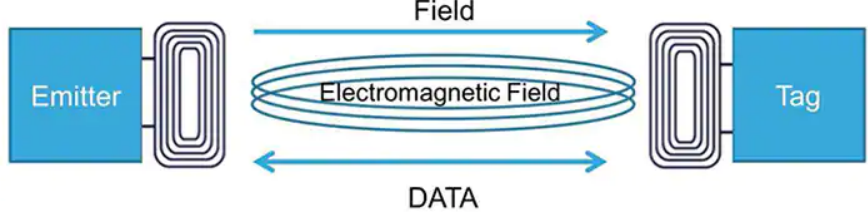
\includegraphics[width=8cm]{Bilder/refart_GPIN}}
   \caption{Teilnehmer der Kommunikation über NFC\\(\cite{refart:GPIN})}
   \label{fig:refart_GPIN}
\end{figure}


\subsubsection{Angriffsmöglichkeit auf NFC}

Da diese Technologie relativ neu ist \cite{refip:NTAS}, sie existiert seit 2006, sind Schwachstellen 
und Härtungsmaßnahmen nicht in ihrer Vollständigkeit bekannt. Drahtlose Verbindungen sind auch für ihre Schattenseite 
bekannt \cite{refip:NYRS}. Maßnahmen zu entwickeln, die sich an verschiedene Systeme anpassen, kosten Zeit 
und Investitionen von Banken und Sicherheitsfirmen. Für jeden möglichen Angriffe müssten Gegenmaßnahmen existieren, 
sodass das Schutzziel der Integrität\footnote{Es ist Subjekten nicht möglich, die zu schützenden Daten unatorisiert und 
unbemerkt zu manipulieren \cite{refbook:SWIS}.} nicht verletzt wird.

Bekannte Angriffe für kabellose Verbindungen können auch bei NFC verwendet werden\cite{refip:NYRS}, wie die
Erstellung und das Hinzufügen von Dateien in einem Opfersystem mit umfangreichen Privilegien; die Konzipierung
von schwachen digitalen Zertifikaten oder auch die Verwendung von Reverse Engineering\footnote{Reverse
Engineering ist ein Prozess von der Identifzierung von Bestandteilen eines Systems und von die Wiederherstellung 
dieser in einem anderen Format \cite{refart:CHRE}. Im Bereich der Cyber-Security wird Reverse-Engineering 
verwendent, um Schwachstellen von Systemen zu entedecken, sodass diese gegen Hardware und Software ausgenutzt
werden können \cite{refip:CMBM}.}. \cite{refart:ALSI} hebt andere Schwachstellen hervor: 
\textit{Eavesdropping}\footnote{Eavesdropping ist das unauthorisierte Mithören von einer Kummunikation \cite{refbook:SWIS}.}
je nachdem, wie viele Ressourcen investiert werden, kann ein Angreifer in der Lage sein, der Kommunikation
zu lauschen; \textit{Denial-of-Service}\footnote{Bei solchen Angriffen wird die Verfügbarkeit des Dienstes verletzt, 
sodass die Kommunikation nicht mehr einwandfrei stattfinden kann \cite{refbook:SWIS}.}, um die Authentifizierung
und Verfügbarkeit der Kommunikation zu beeinträchtigen.


\subsubsection{Gegenmaßnahmen für die Härtung von drahtlose Verbindung}

Um die Risiken bei der Verwendung von NFC zu abzuschwächen, schlägt \cite{refip:NYRS} einige Sicherheitsmechanismen vor, 
die sich eher auf allgemeine drahtlose Verbindungen beziehen, die auch für NFC verwendet werden können: Nutzung von modernen 
kryptographischen Standards für die Validierung von Zertifikaten; Verwendung von Zwei-Faktor-Authentifizierung; Erstellung
von schwer zu erratenden Passwörtern; Registrierung von authorisierten Geräten; Einsetzung von künstlicher Intelligenz 
(KI) für die Detektion von abweichendem Verhalten; Kontrolle gegen Social Engineering \footnote{Beim Social-Engineering
nutzt der Täter den ``Faktor Mensch'' als vermeintlich schwächstes Glied der Sicherheitskette aus, um seine kriminelle
Absicht zu verwirklichen.\cite{booklet:BSSE}}


 Kredit- und EC-Karten sollen auch als Zahlungsmittel bei unserem Click-and-Buy-Automat akzeptiert werden. 
In Bezug auf diese Zahlungsmittel, wird die Sicherheit im folgenden untersucht.

\subsection{Anwendung von Smartcards und sicheres Bezahlen}
Smartcards sind heutzutage sehr stark verbreitet, nicht nur für eine Zahlungsabwicklung, sondern auch für die Identifizierung.
Viele Ausweise wie zum Beispiel der Reisepass und die Krankenkassenkarte verwenden diese Technologie zur Authentifizierung
des Nutzenden. Im folgenden ist ein Beispiel von einer Smartcard für eine zahlende Karte zu sehen: 

\begin{figure}[H]
   \centering{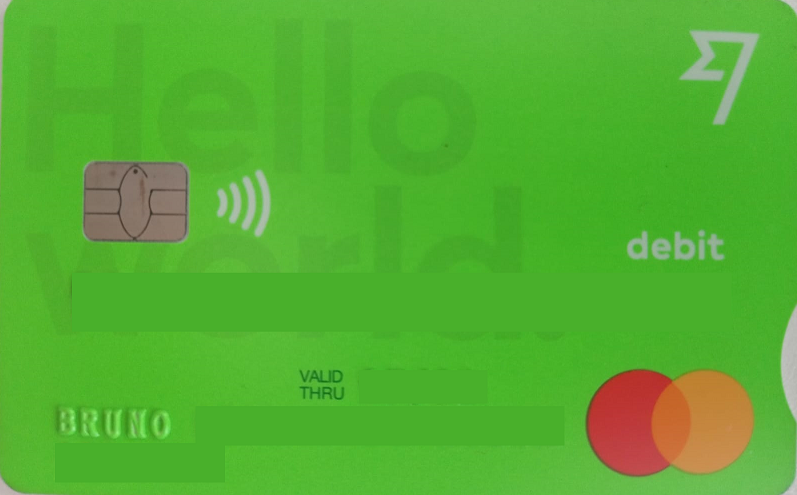
\includegraphics[width=4cm]{Bilder/eigenes_Bild_Karte.png}}
   \caption{Eine Smartcard und deren eingebetete Mikrochip\\(eigene Quelle)}
   \label{fig:eigenes_Bild}
\end{figure}

Die Smartcard wurde vor mehr als 40 Jahren erfunden und ihr Ziel ist die Sicherheit von Kartenzahlungen und allgemeine
Authentifizierungsverfahren zu erhöhen \cite{refip:JFSB}. Sie unterscheiden sich von traditionelen 
Magnetstreifenkarten, weil sie verschiedene Authentifizierungsmethoden ermöglichen auch ohne eine direkte 
Verbindung zur Bank \cite{refbook:ATMS}. Im folgenden wird der Authentifizierungsprozess einer Smartcard 
\ref{fig:refbook_ATMS} dargestellt. 

\vfill
%htb
\begin{figure}[H]
    \centering{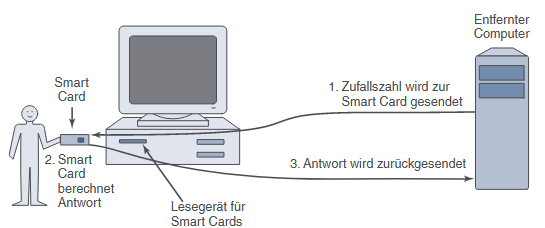
\includegraphics[width=6cm]{Bilder/refbook_ATMS.png}}
   \caption{Authentifizierungsprozess von Smartcards\\(Tanenbaum, 2009, S.755)}
   \label{fig:refbook_ATMS}
\end{figure}
\vfill

Die meisten Angriffe bei Smartcards geschehen laut \cite{refmas:ASSS} auf Hardwareebene. Er beschreibt folgende 
Techniken für Angriffe: Protokollanalyse, bei schwacher Konzipierung oder mangelnder Verschlüsselung ermöglichen Zugang 
zum Klartext; Hardware Reverse Engineering: Verständnis über die Algorithmen oder Extrahieren des Schlüssels


\subsubsection{Angriffsmöglichkeit auf Smartcards}
Smartcards sind auf Hardwareebene extrem sicher. \cite{refmas:ASSS} bezeichnet sie auch als ein in Hardware gegossener
Tresor für Informationen. Wenn eine Smartcard für das Bezahlen verwendet wird, ist kein Backend-System nötig,
denn alle wichtigen Informationen wie das Guthaben sind direkt auf der Karte gespeichert. Aus diesem Grund können
keine Daten abgefangen werden, die auf dem Weg vom Lesegerät zum Backend-System sind, was den Bezahlprozess
deutlich sicherer macht. Zudem muss jede Kommunikation vom Lesegerät initiiert werden, die Karte selber startet
also in keinem Fall eine Kommunikation. Da die wichtigsten Daten direkt auf der Karte gespeichert sind, muss ein Angriff
auf die Hardware initiiert werden, um an relevante Informationen zu gelangen. Eine weitere Möglichkeit wäre,
die Schwachstellen eines bestimmten Protokolls, das für die Kommunikation verwendet wird auszunutzen.

\subsubsection{Gegenmaßnahmen für die Härtung von Smartcards}
Um einen Angriff auf die Hardware möglichst zu vermeiden, ist es sinnvoll den Chip nicht rekonstruierbar zu machen,
das heißt es werden keine Standardzellen oder ähnliches verwendet. Zusätzlich spielt die Verschlüsselung 
der Daten eine große Rolle und erhöht die Sicherheit enorm. Außerdem können Mechanismen in die Smartcard 
eingebaut werden, die permanent die Spannung oder Frequenz überprüfen und sobald etwas
nicht dem Normalzustand entspricht, wird der Chip ausgeschaltet, sodass kein Lesegerät mit der 
Karte kommunizieren kann. Letztlich ist es wichtig, dass jede Karte individuell ist, sodass ein 
erfolgreicher Angriff kein Sicherheitsrisiko für andere Karten darstellt \cite{refmas:ASSS}. 
Dazu wären asymmetrische Verschlüsselungsverfahren sinnvoller als symmetrische, da jede Karte bei
asymmetrischer Verschlüsselung einen öffentlichen und privaten Schlüssel hat und nicht alle den
selben Schlüssel haben.




%- Smartcards sind auf der Hardwareebene extrem sicher. \cite{refmas:ASSS}  bezeichent Smartcards auch als 
%  ein in Hrdware gegossener Tresor für Informationen. 
%- das Guthaben oder der Verfügungsrahmen wird direkt auf der Karte gespeichert, sodass der ganze Prozess nicht über ein Backend-System laufen muss
%- die Komunikation wird immer vom Leser initiiert, die Karte reagiert nur
%- Angriffe richten sich direkt gegen die Hardware, nicht etwa Socail Engineering 
%- Analyse von übertragenen Daten --> Rückschlüsse auf Schwachstellen vom verwendeten Protokoll
%
%Gegenmaßnahmen:
%- damit der Chip nicht rekonstruierbar ist, sollte dieser möglichst Komplex sein, keine Standardzellen oder ähnliches einbauen
%- Zusätzlich lassen sich die Inhalte von Bussen und Speichern bereits auf Hardwareebene
%  durch Scrambling, das heißt das Vertauschen von Adressen, oder durch Verschlüsselung
%  der Daten schützen [2, S.540f][2, S.544f]. Schutzschichten, die den gesamten Chip umgeben
%  und von diesem permanent auf ihre Unversehrtheit geprüft werden, bilden eine weitere
%  Barriere die interne Funktionsweise zu analysieren [2, S.539f]. Andere Sensoren, etwa
%  zur Überwachung von Spannung oder Frequenz, können den Chip abschalten, sobald
%  diese einen Betrieb außerhalb der zulässigen Spezifikationen und damit einen möglichen
%  Angriff erkennen
%- Seitenkanal Angriffe können zum Beispiel durch immer gleich bleibenden Stromverbrauch verhindert werden
%- Grundvoraussetzung für ein sicheres System ist eine Authentifizierung der jeweiligen
%  Gegenstelle bei der Kommunikation, da nur so sicher gestellt werden kann, dass es sich
%  beim Kommunikationspartner nicht um einen Angreifer handelt [2, S.571]. Obwohl es
%  auch möglich ist, allein die Integrität übertragener Daten zu schützen, werden diese
%  oftmals zusätzlich verschlüsselt, sodass auch die Vertraulichkeit gewährleistet ist [2, S.570].
%  Alle für derartige kryptografische Operationen eingesetzten Algorithmen sollten öffentlich
%  bekannt und untersucht sein, um Sicherheitslücken soweit wie möglich auszuschließen [30,
%  S.9].
%  Bei der Implementierung der Algorithmen ist darauf zu achten, dass ein konstantes
%  Zeitverhalten gewährleistet wird, das heißt unabhängig von den Eingabedaten die gleiche
%  Ausführungszeit benötigt wird, um so darauf basierende Seitenkanalattacken zu unterbin-
%  den [2, S.560f]. Zufallszahlen, die unter anderem bei der Authentifizierung eine wichtige
%  Rolle spielen, sind auf kryptografisch sichere Weise zu erzeugen
%- Auf organisatorischer Ebene ist es wichtig, die Verwendung von kartenindividuellem
%  Schlüsselmaterial sicherzustellen, um zu verhindern, dass ein erfolgreicher Angriff auf
%  eine Karte auch andere Karten unmittelbar gefährdet. Dies geschieht entweder durch den
%  Einsatz asymmetrischer Kryptografie, bei der für jede Karte eigenes Schlüsselmaterial
%  generiert und von einer zentralen Instanz signiert wird, oder durch die so genannte
%  Key Diversification bei Verwendung symmetrischer Kryptografie. Hierbei wird unter
%  Einsatz einer Einwegfunktion ein kartenindividueller Schlüssel von einem Hauptschlüssel
%  abgeleitet und nur der abgeleitete Schlüssel auf der Karte gespeichert [30, S.22].
%  Sollte es zu einem Verlust oder einem erfolgreichen Angriff auf eine Karte kommen,
%  muss es möglich sein, diese Karte (genauer: ihr Schlüsselmaterial) im System zu sperren,
%  indem entsprechende Sperrlisten gepflegt werden [2, S.572]. Dass eine Karte angegriffen
%  und beispielsweise geklont wurde, lässt sich durch das Erstellen von Logeinträgen für
%  jede Verwendung und deren Überprüfung auf Unregelmäßigkeiten erkennen

\subsection{Fazit}

NFC ist eine Technologie die viele Vorteile bietet. Sie ermöglicht in nur einem Gerät die Anwendung verschiedener
Aktivitäten, wie Zahlung, Identifizierung und Authentifizierung, ohne dass ein Nutzer unterschiedliche Karten bei sich haben muss. Die 
Nachteile beziehen sich auf die Neuigkeit dieser Technologie, die mehr Forschung verlangt, damit deren Schachstelle weiter erforscht
werden \cite{refart:ALSI}.  Die Technologie der Smartcards ist bereits breit erforscht, sodass sowohl Schwachstellen, als auch 
Härtungsmaßnahmen bekannt sind. Die Akzeptanz und die Verwendung von Smartcards sind auch
umfangreicher, besonders weil auch Non-Native sie eher nutzen.

Aus den obigen genannten Gründen können wir sagen, dass Smartcards der bessere Einsatz für einen Click-and-Buy-Automat
neben einem Campingplatz wäre, solange die Technologie von NFC noch nicht so weit erforscht ist und in der Gesellschaft nicht so etabliert ist.
